\documentclass[english,notitlepage,letterpaper, 10pt]{article} % para articulo en castellano
\usepackage{cite}
\usepackage[utf8]{inputenc} % Acepta caracteres en castellano
\usepackage[english]{babel} % silabea palabras castellanas
\usepackage{amsmath}
\usepackage{here}
\usepackage{multirow}

\usepackage{amsfonts}
\usepackage{amssymb}
\usepackage{hyperref} % navega por el doc
\usepackage{graphicx}
\usepackage{geometry}      % See geometry.pdf to learn the layout options.
\geometry{letterpaper}                   % ... or a4paper or a5paper or ... 
%\geometry{landscape}                % Activate for for rotated page geometry
%\usepackage[parfill]{parskip}    % Activate to begin paragraphs with an empty line rather than an indent
\usepackage{epstopdf}
\usepackage{fancyhdr} % encabezados y pies de pg

\usepackage{listings}
\usepackage{color}

\definecolor{dkgreen}{rgb}{0,0.6,0}
\definecolor{gray}{rgb}{0.5,0.5,0.5}
\definecolor{mauve}{rgb}{0.58,0,0.82}

\lstset{frame=shadowbox,
  language=Matlab,
  aboveskip=3mm,
  belowskip=3mm,
  showstringspaces=false,
  columns=flexible,
  basicstyle={\small\ttfamily},
  numbers=left,
  numberstyle=\tiny\color{gray},
  keywordstyle=\color{blue},
  commentstyle=\color{dkgreen},
  stringstyle=\color{mauve},
  breaklines=true,
  breakatwhitespace=true
  tabsize=3
  rulesepcolor=\color{blue}
}

\newcommand{\university}{\normalsize Universidad Industrial de Santander}
\newcommand{\faculty}{\normalsize  Escuela de Ingenier\'ia de Sistemas e Inform\'atica}
\newcommand{\codigo}{\normalsize  2182066}
\newcommand{\grupo}{\normalsize  B2}
\pagestyle{fancy} 
\chead{\bfseries Lab. } 
\lhead{} % si se omite coloca el nombre de la seccion
\rhead{\today} 
\lfoot{\it  An\'alisis N\'umerico } 
\cfoot{\university} 
\rfoot{\thepage} 

\voffset = -0.25in 
\textwidth = 7.5in
\textheight = 9in
\oddsidemargin = -0.6in
\headheight = 20pt 
\headwidth = 7.5in
\renewcommand{\headrulewidth}{0.5pt}
\renewcommand{\footrulewidth}{0,5pt}
\DeclareGraphicsRule{.tif}{png}{.png}{`convert #1 `dirname #1`/`basename #1 .tif`.png}


\begin{document}

\title{	\vspace{-12mm}
\includegraphics[width=0.2\linewidth]{Logos/UIS.pdf}\\Informe Laboratorio: An\'alisis Num\'erico\\  \centering Pr\'actica No. 2}
\author{
\textbf{Daniel Delgado} \\ \textbf{C\'odigo:} \codigo\\
\textbf{Grupo:} B2\\
\textit{\faculty}\\
\textit{\university}}
\date{\today}
\maketitle

\section{Introducci\'on}

Las raíces de las funciones, de manera general, forman parte de las herramientas con las cuales es posible resolver problemas que parten desde la determinación de las condiciones iniciales de un modelo matemático, hasta la determinación de puntos los cuales describen trayectorias de sistemas físicos. 

La necesidad de hacer este típo de cálculos, junto con el avance de la computación, y las posibilidades de emplear estos recursos en el cálculo de las raíces, dió origen a algunos métodos los cuales permitían realizar este cálculo de manera simple. El método de bisección, parte de estos métodos, permite el cálculo de raíces dentro de un intervalo dado a partir del uso de puntos medios. 

La compresión de este concepto, al igual que el desarrollo de la algoritmia relacionada, son los principales temas a a tratar durante el desarrollo del presente informe, así como la resolución de los problemas propuestos a manera de pregunta orientadora durante el desarrollo del componente práctico del mismo.

\section{Desarrollo}

  \begin{enumerate}
    \item \textbf{Preguntas Propuestas}
    
    De manera inicial, la guía de laboratorio propone las siguientes preguntas con el fin de llevar
    más allá la comprensión de los conceptos trabajados durante el desarrollo práctico del laboratorio.

    \begin{enumerate}

      \item Explique brevemente qué es el método de bisección\\
      El método de bisección, en términos simples, consiste en tomar 2 puntos, uno que evaluado en la función sea positivo, y otro negativo, entre los cuales se cree tener la raíz de una función. A partir de esto, se calculará el punto medio entre los 2 puntos escogidos; el punto encontrado se computará en la función y, dependiendo de si el resultado es positivo o negativo, el nuevo punto será tomado como un nuevo punto externo. Este proceso se repetirá hasta que se encuentre un punto en el cual este, evaluado en la función, de 0. 

      \item ¿Qué condiciones deben cumplir los puntos a y b para ser usados satisfactoriamente en el método de bisección? \\
      De manera básica, la condición básica la cual deben cumplir los puntos a y b es que, el producto de estos puntos evaluados en la función sea menor que 0, es decir $g(a) \times g(b) < 0$. En el caso de que se cumpla, los puntos pueden ser candidatos para aplicar el método de bisección.

      \item Describa el paso de decisión en cada iteración del método de bisección \\
      En cada iteración el primer paso consta de calcular el punto medio entre los puntos que están siendo empleados para calcular la raíz de la función. Tras calcular este, el punto encontrado debe ser evaluado en la función. El resultado de este, en caso de ser 0, nos daría el punto raíz de la función por lo que más iteraciones no serán necesarias. En el caso de que el punto, evaluado en la función, de un valor positivo, este será el nuevo punto a tomar y remplazará el valor del punto de valor positivo anteriormente empleado. Si el punto evaluado tiene valor negativo este remplazará el punto negativo anteriormente usado. Este proceso se repetirá hasta encontrar un punto cuyo valor, evaluado en la función, sea 0.

      \item ¿Qué aplicaciones tiene el método de bisección? \\
      La principal aplicación del método de bisección, de manera general, es el encontrar raíces para muchas funciones de manera iterativa. Esto permite, de manera simple, la posibilidad de computar raíces complicadas con un alto grado de precisión en el caso de ser necesario.

    \end{enumerate}

    \item \textbf{Aplicando}
    
    Con el fin de comprender el como se aplica el método de bisección de manera manual, se desarrollará una prueba de escritorio con la cual se permite mejorar la comprensión del funcionamiento del método.

    \begin{table}[H]

      \centering
      Punto inicial a: $1$ Punto final b: $3$ \\
      \vspace{0.5cm}
      \begin{tabular}{|p{2.5cm}|p{2.5cm}|p{2.5cm}|p{2.5cm}|p{2.5cm}|p{2.5cm}|}

       \hline  
       $k$ & $a_k$ & $c_k$ & $b_k$ & $f(c_k)$ & $|\frac{c_k-c_{k+1}}{c_k}|$ \\ \hline
       0 & 1     & 2      & 3       & 2.7744   & 0.25   \\ \hline
       1 & 2     & 2.5    & 3       & -1.942   & 0.1    \\ \hline
       2 & 2     & 2.25   & 2.5     & -0.7158  & 0.0555 \\ \hline
       3 & 2     & 2.125  & 2.25    & 0.48568  & 0.0294 \\ \hline
       4 & 2.125 & 2.1875 & 2.25    & -0.19785 & 0.0142 \\ \hline
       5 & 2.125 & 2.1563 & 2.1875  & 0.11877  & 0.0072 \\ \hline

      \end{tabular}
    \end{table}

    \item \textbf{Implementando}
    
    Una de las partes más importantes respecto al desarrollo del trabajo de laboratorio en cuanto a su componente práctico se requiere a la implementación de algoritmia con el fin de cumplir con un objeto o dar solución a un problema propuesto.

    \begin{enumerate}

      \item Búsqueda de intervalos
      
      En primera medida, la necesidad de una función capaz de determinar intervalos de puntos en los cuales existan raíces las cuales puedan ser calculadas por el método de bisección era de alta importancia.
      
      Con esto en mente, se desarrolló la función \texttt{intervalFinder(aFunction)}. Esta función, en términos generales, realiza una búsqueda aplicando un \textit{brute-force attack}, es decir, que busca un intervalo válido utilizando prueba y error hasta que encuentra dicho intervalo.

      \begin{lstlisting}
function [output] = intervalFinder(aFunction)
    if isa(aFunction,'function_handle')

        negTracer = 0;
        posTracer = 0;
        
        lowerIndex = 1;
        upperIndex = 1500;
        
        for index = lowerIndex:upperIndex        
            negLead = index*(-1)-1;
            posLead = index+1;
            
            if aFunction(negLead)*aFunction(negTracer) < 0
                output = [negLead negTracer];
                return;
            elseif aFunction(posTracer)*aFunction(posLead) < 0
                output = [posTracer posLead];
                return;
            else
                %do nothing, keep the loop
            end

            negTracer = index*(-1);
            posTracer = index;
        end
    disp('Interval not found!')    
    else
        disp('Given parameters are invalid! Check params and try again')
    end
end
      \end{lstlisting}

      En términos simples, la función \texttt{intervalFinder(aFunction)}, iniciando desde 0, se extiende hacia los valores positivos y negativos del dominio de la función. Esto es evidenciado en las líneas presentes en el ciclo iterativo el cual es el responsable de recorrer todo el espectro. 
      
      Algo a resaltar de esta función son sus limitaciones. Esta implementación, aunque simple en su lógica, no es particularmente complicada, es bastante limitada en cuanto a encontrar valores. Esto se debe al como el índice es usado para determinar el intervalo a evaluar. Al ser valores enteros, en el caso de que la raíz se encuentre en uno de estos, cabe la posibilidad de que este sea ignorado. Sin embargo, debido a lo verdaderamente compleja que es la tarea de determinar intervalos válidos, es lo más apto para la tarea a resolver.

      \item Aplicando el método de bisección
      
      Con el fin de aplicar el método de bisección, y satisfactoriamente completar los objetivos del laboratorio, se desarrolló la función \texttt{bisection(aFunction,lowerBracket,upperBracket,iterarions)}. Esta función, básicamente, realiza la búsqueda de las raíces de una función dada con un número de iteraciones definidas.

      \begin{lstlisting}
function output = bisection(aFunction, lowerBracket, upperBracket, iterarions)
    if (isa(aFunction,'function_handle') && (lowerBracket < upperBracket) && (aFunction(lowerBracket)*aFunction(upperBracket) < 0) && (iterarions > 0))
        disp(['Given parameters are valid!', newline, 'Calculating roots of ', func2str(aFunction)])

        bisector = @(a,b) (a+b)/2;
        if aFunction(lowerBracket) < 0
            lowerBound = lowerBracket;
            upperBound = upperBracket;
        else
            lowerBound = upperBracket;
            upperBound = lowerBracket;
        end
        
        for index = 1:iterarions
            newBound = bisector(lowerBound,upperBound);
            newRange = aFunction(newBound);
            if newRange == 0
                disp(['A root for ', func2str(aFunction), ' was found! Root for function is ', num2str(newBound), ' (Root found after ', num2str(index), ' iterarions)']);
                output = newBound;
                return;
            elseif newRange < 0
                lowerBound = newBound;
            else %newRange > 0
                upperBound =  newBound;
            end
        end

        if (aFunction(newBound) == 0)
            disp(['A root for ', func2str(aFunction), ' was found! Root for function is ', num2str(newBound)])
            output = newBound;
        elseif (abs(aFunction(newBound)) < 0.00001)
            disp(['A possible root was found close to ', num2str(newBound), '. More iterations might confirm if it is a root.'])
            output = newBound;
        else
            disp('A root was not found. Increasing the number of iterations could help locating one but it is not completely certain.')
            output = NaN;
        end
    else 
        disp('Given parameters are invalid! Check params and try again')
    end
end
      \end{lstlisting}

      \texttt{bisection} aplica el proceso básico requerido para determinar las raíces de una función. De manera inicial, tras validar los parámetros dados, la función determina cual de los extremos del intervalo dado es el negativo y los asigna correspondientemente con el fin de universalizar el tratamiento de los datos. Tras esto, se iniciará un ciclo iterativo en el cual se encontrará el punto medio del intervalo actual al igual que el valor de dicho punto al ser evaluado en la función. Tras esto, se buscará saber si una raíz ha sido encontrada; de ser así, se pasará el valor encontrado y cerrará el ciclo iterativo. Por el contrario, se determinará en que lado del intervalo debe ir el nuevo valor. Finalmente, se dará el output de la función en el caso de que se haya encontrado la raíz o un valor muy cercano a este.

      Con el fin de probar el funcionamiento de \texttt{bisection.m}, ejecutó la función con los siguientes parámetros:

      \begin{lstlisting}
f = @(x)x^2-x-1;
lowerBracket = 1;
upperBracket = 6;
ite = 100;
bisection(f,lowerBracket,upperBracket,ite);
      \end{lstlisting}

      El resultado de la ejecución, tras 53 iteraciones $ans =  1.618033988749895$.

      \item Teoría vs práctica
      
      Una de las herramientas que se tienen disponibles en cuanto al desarrollo de la parte iterativa, es el cálculo teórico de la cantidad de iteraciones. Este cálculo puede, parcialmente, realizarse con la siguiente inecuación:

      \begin{center}
        \scalebox{1.1}{$\varepsilon \leq \frac{b-a}{2^{n+1}}$}
      \end{center}

      Esta inecuación hace referencia al error absoluto, donde a y b son los límites del intervalo trabajado, n a la cantidad de iteraciones y $\varepsilon$ al error admisible. Convirtiendo la desigualdad en una igualdad, podemos determinar una cantidad teórica de iteraciones en las cuales, para un intervalo determinado, se debería aproximar a la raíz aplicando el método de bisección. Tras despejar para n, y aplicar la función techo para evitar subestimar y volver enteros los resultados, tendremos como resultado la siguiente ecuación:
      \begin{center}
        \scalebox{1.1}{$n = \lceil \log_2(\frac{b-a}{\varepsilon})-1 \rceil$}
      \end{center}

      A partir de esto, podemos determinar la cantidad de iteraciones teóricas para cada uno de los errores admisibles propuestos. En el caso de la función $f(x)=(x-8)(x-3)^2$, se buscará la raíz relacionada con el primer término de la expresión, es decir, $x=8$. 
      
      \begin{table}[H]
        \centering
        \begin{tabular}{|c|c|c|c|c|c|c|}
        \hline
        \multirow{3}{*}{a=4}  & \multirow{2}{*}{$\varepsilon$} & \multirow{2}{*}{$1e^{-2}$} & \multirow{2}{*}{$1e^{-4}$} & \multirow{2}{*}{$1e^{-6}$} & \multirow{2}{*}{$1e^{-8}$} & \multirow{2}{*}{$1e^{-10}$} \\ &  &  &  &  &  &   \\
        \cline{2-7}  & \multirow{2}{*}{n teórico} & \multirow{2}{*}{9} & \multirow{2}{*}{15}& \multirow{2}{*}{22}& \multirow{2}{*}{29}& \multirow{2}{*}{35} \\ \cline{1-1} \multirow{3}{*}{b=10} &  &  &  &  &  &   \\
        \cline{2-7} & \multirow{2}{*}{n práctico} & \multirow{2}{*}{13}  & \multirow{2}{*}{19}  & \multirow{2}{*}{26}  & \multirow{2}{*}{33}  & \multirow{2}{*}{39}\\ &  &  &  &  &  &  \\ \hline
        \end{tabular}
      \end{table}

      De esto, podemos generar la siguiente gráfica (Fig. \ref{leGraph}).

      \begin{figure}[H]
        \centering
        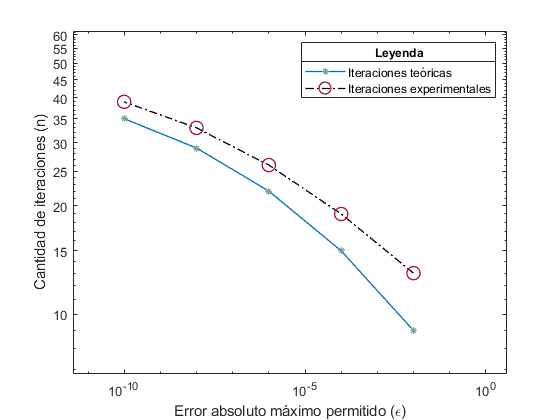
\includegraphics[width=10cm]{Images/leGraph.png}
        \caption{Comparación de las iteraciones teóricas contra las prácticas}
        \label{leGraph}
      \end{figure}

      De esto, podemos ver que, aunque los valores no sean particularmente distantes en términos computacionales, existe un desfase constante de entre 6 y 7 iteraciones de diferencia. Esto puede ser debido a varias cosas pero, de manera principal, puede deberse a la implementación de la función \texttt{bisection} que, aunque cumple su cometido, no sea la manera más eficiente de encontrar las raíces de una función.

      \item Aplicando de manera visual
      
      La necesidad de realizar comprobaciones visuales de la ejecución de una función es algo que siempre es deseable debido a que simplifica la interpretación de los datos presentados. Con el fin de cumplir esto, se desarrolló una versión modificada de \texttt{bisection}, \texttt{visualBisection.m}, la cual muestra de manera visual el como se va moviendo el punto medio.

      \begin{lstlisting}
function output = visualBisection(aFunction, lowerBracket, upperBracket, iterarions)
    if (isa(aFunction,'function_handle') && (lowerBracket < upperBracket) && (aFunction(lowerBracket)*aFunction(upperBracket) <= 0) && (iterarions > 0))
        disp(['Given parameters are valid!', newline, 'Calculating roots of ', func2str(aFunction)])

        fplot(aFunction, [lowerBracket-0.1 upperBracket+0.1], 'Color', 'black')
        line([lowerBracket-0.1 upperBracket+0.1], [0 0], 'Color', 'black')
        
        bisector = @(a,b) (a+b)/2;
        
        if aFunction(lowerBracket) < 0
            lowerBound = lowerBracket;
            upperBound = upperBracket;
        else
            lowerBound = upperBracket;
            upperBound = lowerBracket;
        end
        
        for index = 1:iterarions
            newBound = bisector(lowerBound,upperBound);
            newRange = aFunction(newBound);
            if newRange == 0
                disp(['A root for ', func2str(aFunction), ' was found! Root for function is ', num2str(newBound), ' (Root found after ', num2str(index), ' iterarions)']);
                output = newBound;
                line([newBound newBound], ylim, 'Color', rand(1,3));
                return;
            elseif newRange < 0
                lowerBound = newBound;
                line([newBound newBound], ylim, 'Color', rand(1,3));
            else %newRange > 0
                upperBound =  newBound;
                line([newBound newBound], ylim, 'Color', rand(1,3));
            end
        end

        if (aFunction(newBound) == 0)
            disp(['A root for ', func2str(aFunction), ' was found! Root for function is ', num2str(newBound)])
            output = newBound;
        elseif (abs(aFunction(newBound)) < 0.00001)
            disp(['A possible root was found close to ', num2str(newBound), '. More iterations might confirm if it is a root.'])
            output = newBound;
        else
            disp('A root was not found. Increasing the number of iterations could help locating one but it is not completely certain.')
            output = NaN;
        end
    else    
        disp('Invalid params! Check entries!')
    end
end
      \end{lstlisting}

      La principal diferencia con respecto a la función original, es que, además de graficar cada la función dada, grafica cada línea por la que el punto medio es calculado.

      En pos de probar el funcionamiento de \texttt{visualBisection}, se ejecutó bajo los siguientes parámetros:
      
\begin{lstlisting}
f = @(x)(tan(x).^2)-x;
lowerBracket = 2;
upperBracket = 3;
ite = 7;
visualBisection(f,lowerBracket,upperBracket,ite);
\end{lstlisting}

      Tras la ejecución del código, aunque no se encontró de manera exacta la raíz de la función debido al bajo número de iteraciones, la gráfica resultante de la ejecución, Fig \ref{leBisection}, muestra la progresión de la función.

      \begin{figure}[H]
        \centering
        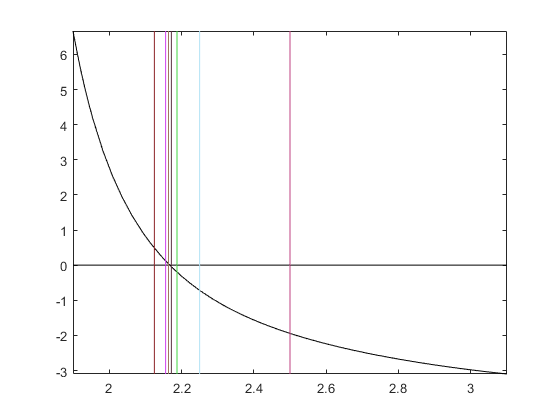
\includegraphics[width=10cm]{Images/leBisection.png}
        \caption{Gráfica resultante de \texttt{visualBisection}}
        \label{leBisection}
      \end{figure}

    \end{enumerate}

    \item \textbf{Interprentado}
  
    Con el fin de demostrar la funcionalidad de el método de bisección, este se utilizará con el fin de dar solución a un problema planeteado.

    El problema planeteado, relacionado con el modelado de crecimiento poblacional, nos da una situación en la cual, para una población indeterminada con 1500 individuos de manera incial, tras un año, gracias a la inmigración y al crecimiento natural de esta, tendrá una población final de 2264 individuos.

    \begin{enumerate}
      \item \textbf{Determinando la ecuación}
      
      La ecuación empleada con el fin de determinar el factor de crecimiento será la misma dada por el ejercicio planeteado. 

      \begin{center}
        \scalebox{1.1}{$N(t) = N_0 e^{\lambda t} + \varphi \frac{e^{\lambda t}-1}{\lambda}$}
      \end{center}

      Donde $N_0$ es la población inicial, $\lambda$ es el factor de crecimiento poblacional, $\varphi$ el coeficiente relacionado con la inmigración y $t$ es el tiempo en años que ha pasado desde el momento inicial.

      De esto, tras remplazar el valor de $\varphi$ en la función por 475, que es el coeficiente de inmigración dado en el planeteamiento del problema al igual que $N_0$ por 1500 que es la población inicial; podemos evaluar la función para $t = 1$.

      \begin{center}
        \scalebox{1.1}{$N(1) = (1500)e^\lambda + (475) \frac{e^\lambda - 1}{\lambda} = 2264$}
      \end{center}

      Con esto, la función poblacional quedaría en términos de lambda, por lo que ahora debemos determinar el factor de crecimiento. 

      \begin{center}
        \scalebox{1.1}{$f(\lambda) = 0 = (1500)e^\lambda + (475) \frac{e^\lambda - 1}{\lambda} - 2264$}
      \end{center}
    
      De esta función, se calculará la raíz con un error de 0.

      \item \textbf{Solución de la ecuación}

      Seguidamente, se le dió solución al problema con el uso de la función \texttt{bisection} con el uso de los siguientes parámetros:

      \begin{lstlisting}
f = @(x) 1500*exp(1)^(x) + (475*(exp(1)^(x)-1))/x - 2264;
low = 0.01;
upp = 1;
ite = 150;

bisection(f,low,upp,ite);
      \end{lstlisting}

      Tras computar esto, podemos ver el como, tras 53 iteraciones realizadas por la función, esta da como resultado $0.154365833565118$, lo cual, al evualuarlo en la función, podemos ver que efectivamente da $0$. Es decir que, para el caso planteado, el factor de crecimiento poblacional para la población, sería $0.154365833565118$.

    \end{enumerate}

  \end{enumerate}         

  
  


\section{Anexos}

\hspace{0.5cm}\texttt{bisection.m}
\begin{lstlisting}
function output = bisection(aFunction, lowerBracket, upperBracket, iterarions)
    %Checks function params%
    if (isa(aFunction,'function_handle') && (lowerBracket < upperBracket) && (aFunction(lowerBracket)*aFunction(upperBracket) <= 0) && (iterarions > 0))
        disp(['Given parameters are valid!', newline, 'Calculating roots of ', func2str(aFunction)])

        bisector = @(a,b) (a+b)/2;
        
        if aFunction(lowerBracket) < 0
            lowerBound = lowerBracket;
            upperBound = upperBracket;
        else
            lowerBound = upperBracket;
            upperBound = lowerBracket;
        end
        
        for index = 1:iterarions
            newBound = bisector(lowerBound,upperBound);
            newRange = aFunction(newBound);
            if newRange == 0
                disp(['A root for ', func2str(aFunction), ' was found! Root for function is ', num2str(newBound), ' (Root found after ', num2str(index), ' iterarions)']);
                output = newBound;
                return;
            elseif newRange < 0
                lowerBound = newBound;
            else %newRange > 0
                upperBound =  newBound;
            end
        end

        if (aFunction(newBound) == 0)
            disp(['A root for ', func2str(aFunction), ' was found! Root for function is ', num2str(newBound)])
            output = newBound;
        elseif (abs(aFunction(newBound)) < 0.00001)
            disp(['A possible root was found close to ', num2str(newBound), '. More iterations might confirm if it is a root.'])
            output = newBound;
        else
            disp('A root was not found. Increasing the number of iterations could help locating one but it is not completely certain.')
            output = NaN;
        end
    else 
        disp('Given parameters are invalid! Check params and try again')
    end
end
\end{lstlisting}


\texttt{stopCritBisection.m}
\begin{lstlisting}
function output = stopCritBisection(aFunction, lowerBracket, upperBracket, iterarions, stopCriteria)
    if (isa(aFunction,'function_handle') && (lowerBracket < upperBracket) && (aFunction(lowerBracket)*aFunction(upperBracket) <= 0) && (iterarions > 0) && stopCriteria >= 0)
        disp(['Given parameters are valid!', newline, 'Calculating roots of ', func2str(aFunction)])

        bisector = @(a,b) (a+b)/2;
        
        if aFunction(lowerBracket) < 0
            lowerBound = lowerBracket;
            upperBound = upperBracket;
        else
            lowerBound = upperBracket;
            upperBound = lowerBracket;
        end
        
        for index = 1:iterarions
            newBound = bisector(lowerBound,upperBound);
            newRange = aFunction(newBound);
            if abs(newRange) < stopCriteria
                disp(['Stop critera met! Root for function is ', num2str(newBound), ' (Root found after ', num2str(index), ' iterarions)']);
                output = newBound;
                return;
            elseif newRange < 0
                lowerBound = newBound;
            else %newRange > 0
                upperBound =  newBound;
            end
        end

        if (aFunction(newBound) == 0)
            disp(['A root for ', func2str(aFunction), ' was found! Root for function is ', num2str(newBound)])
            output = newBound;
        elseif (abs(aFunction(newBound)) < 0.00001)
            disp(['A possible root was found close to ', num2str(newBound), '. More iterations might confirm if it is a root.'])
            output = newBound;
        else
            disp('A root was not found. Increasing the number of iterations could help locating one but it is not completely certain.')
            output = NaN;
        end
    else 
        disp('Given parameters are invalid! Check params and try again')
    end
end
\end{lstlisting}


\texttt{visualBisection.m}
\begin{lstlisting}
function output = visualBisection(aFunction, lowerBracket, upperBracket, iterarions)
    if (isa(aFunction,'function_handle') && (lowerBracket < upperBracket) && (aFunction(lowerBracket)*aFunction(upperBracket) <= 0) && (iterarions > 0))
        disp(['Given parameters are valid!', newline, 'Calculating roots of ', func2str(aFunction)])

        bisector = @(a,b) (a+b)/2;
        plot([lowerBracket upperBracket],aFunction([lowerBracket upperBracket]))
        
        if aFunction(lowerBracket) < 0
            lowerBound = lowerBracket;
            upperBound = upperBracket;
        else
            lowerBound = upperBracket;
            upperBound = lowerBracket;
        end
        
        for index = 1:iterarions
            newBound = bisector(lowerBound,upperBound);
            newRange = aFunction(newBound);
            if newRange == 0
                disp(['A root for ', func2str(aFunction), ' was found! Root for function is ', num2str(newBound), ' (Root found after ', num2str(index), ' iterarions)']);
                output = newBound;
                line([newBound newBound], ylim);
                return;
            elseif newRange < 0
                lowerBound = newBound;
                line([newBound newBound], ylim);
            else %newRange > 0
                upperBound =  newBound;
                line([newBound newBound], ylim);
            end
        end

        if (aFunction(newBound) == 0)
            disp(['A root for ', func2str(aFunction), ' was found! Root for function is ', num2str(newBound)])
            output = newBound;
        elseif (abs(aFunction(newBound)) < 0.00001)
            disp(['A possible root was found close to ', num2str(newBound), '. More iterations might confirm if it is a root.'])
            output = newBound;
        else
            disp('A root was not found. Increasing the number of iterations could help locating one but it is not completely certain.')
            output = NaN;
        end
    else    
        disp('Invalid params! Check entries!')
    end
end
\end{lstlisting}


\texttt{intervalFinder.m}
\begin{lstlisting}
function [output] = intervalFinder(aFunction)
    if isa(aFunction,'function_handle')

        negTracer = 0;
        posTracer = 0;
        
        lowerIndex = 1;
        upperIndex = 1500;
        
        for index = lowerIndex:upperIndex        
            negLead = index*(-1)-1;
            posLead = index+1;
            
            if aFunction(negLead)*aFunction(negTracer) < 0
                output = [negLead negTracer];
                return;
            elseif aFunction(posTracer)*aFunction(posLead) < 0
                output = [posTracer posLead];
                return;
            else
                %do nothing, keep the loop
            end

            negTracer = index*(-1);
            posTracer = index;
        end
    disp('Interval not found!')    
    else
        disp('Given parameters are invalid! Check params and try again')
    end
end
\end{lstlisting}

bisectionRunner.m
\begin{lstlisting}
f = @(x)x^2-x-1;
lowerBracket = 1;
upperBracket = 6;
ite = 100;
bisection(f,lowerBracket,upperBracket,ite);
\end{lstlisting}

visualRunner.m
\begin{lstlisting}
f = @(x)(tan(x).^2)-x;
lowerBracket = 2;
upperBracket = 3;
ite = 7;
visualBisection(f,lowerBracket,upperBracket,ite);
\end{lstlisting}

\end{document}  


